% TEX STUDIO MAGIC-COMMENT
% !TeX document-id = {9278c550-dabb-445e-88fc-9cdae0cf3529}
% !TeX root = paper.tex
%%% ↑ TeXのファイル名にあわせて変える
% !TeX encoding = utf8
% !TeX spellcheck = none
% !TeX TXS-program:latex = ptex2pdf -u -l -ot "-synctex=1 -halt-on-error -interaction=nonstopmode" %.tex
% !TeX TXS-program:dvipdf = dvipdfmx %.dvi
% !TeX TXS-program:compile = txs:///latex
% !TeX TXS-program:quick = txs:///compile | txs:///view-pdf-internal --embedded


%%%-------------------------------------------------------------------------
%%% PD3レポートテンプレート
%%% 作成: 金沢工大・情報工学科・鷹合研究室
%%%-------------------------------------------------------------------------

\documentclass[a4paper,dvipdfmx,uplatex,openright]{jsbook}
\usepackage{takagolab}	% 鷹合研の設定

\begin{document}
% !TeX root = paper.tex

\begin{titlepage}
 \begin{center}
  ~\\
  \vspace{1cm}
  {\Large 
  令和98年度\\
 プロジェクトデザインIII\\
  プロジェクトレポート\\
情報工学科\\}
  \vspace{1.3in}
  {\Huge \gtfamily
ベクトルメディアンフィルタと\\
その発展型フィルタを用いた\\
劣化画像の復元\\
  }
  \vspace{2in}
  {\LARGE 
  提出日~~~令和99年~99月~99日\\
  \vspace{0.4in}
  指導教員~:~鷹合 大輔 准教授\\
 \vspace{0.9in}
  氏名 学籍番号 (クラス--名列番号)\\
  \vspace{2mm}
  北野 大地 1234567 (4EP5--90)\\
  奥野 細道 1234568 (4EP5--98)\\
  岡山 桃子 1234569 (4EP5--91)\\
  }
 \end{center}
\end{titlepage}
 %タイトル
\frontmatter % タイトルの次に1ページの空きページを
% !TeX root = paper.tex


\begin{center}
		{\gtfamily \Large 概要}
\end{center}
\vspace{1cm}
\thispagestyle{empty}	
%%%%%%%%%%%%%%%%%%%%%%%%%%%%%%% 概要ここから



○○○○
 ○○○○○○○○○○○○○○○○○○○○○○○○○○○○○○○○○○○○○○○○○○○○○○○○○○○○○○○○ ○○○○ ○○○○○○○○○○○○○○○○○○○○○○○○○○○○○○○○○○○○○○○○○○○○○○○○○○○○○○○○ ○○○○○○○○○○○○○○○○○○○○○○○○○○○○○○○○○○○○○○○○○○○○○○○○○○○○○○○○ ○○○○○○○○○○○○○○○○○○○○○○○○○○○○○○○○○○○○○○○○○○○○○○○○○○○○○○○○ ○○○○○○○○○○○○○○○○○○○○○○○○○○○○○○○○○○○○○○○○○○○○○○○○○○○○○○○○ ○○○○○○○○○○○○○○○○○○○○○○○○○○○○○○○○○○○○○○○○○○○○○○○○○○○○○○○○ ○○○○○○○○○○○○○○○○○○○○○○○○○○○○○○○○○○○○○○○○○○○○○○○○○○○○○○○○ ○○○○○○○○○○○○○○○○○○○○○○○○○○○○○○○○○○○○○○○○○○○○○○○○○○○○○○○○○○○○○○○○○○○○○○○○○○○○○○○○○○○○○○○○○○○○○○○○○○○○○○○○
概要には目的,背景,手法,実験方法,実験結果を簡潔にまとめたものを書く(つまり,論文を1ページに圧縮したものである.概要だけを読んでも,大まかに何をやって,どのような結果になったかが分かるように書くこと.0.5ページ分くらいはうめること.).○○○○ ○○○○○○○○○○ ○○○○○○○○○○○○○○○○○○○○○○○○○○○○○○○○○○○○○○○○○○○○○○○○○○○○○○○○ ○○○○○○○○○○○○○○○○○○○○○○○○○○○○○○○○○○○○○○○○○○○○○○○○○○○○○○○○ ○○○○○○○○○○○○○○○○○○○○○○○○○○○○○○○○○○○○○○○○○○○○○○○○○○○○○○○○ ○○○○○○○○○○○○○○○○○○○○○○○○○○○○○○○○○○○○○○○○○○○○○○○○○○○○○○○○ ○○○○○○○○○○○○○○ ○○○○○○○○○○○○○○○○○○○○○○○○○○○○○○○○○○○○○○○○○○○○○○○○○○○○○○○○ ○○○○○○○○○○○○○○○○○○○○○○○○○○○○○○○○○○○○○○○○○○○○○○○○○○○○○○○○ ○○○○○○○○○○○○○○○○○○○○○○○○○○○○○○○○○○○○○○○○○○○○○○○○○○○○○○○○ ○○○○○○○○○○○○○○○○○○○○○○○○○○○○○○○○○○○○○○○○○○○○○○○○○○○○○○○○○○○○○○○○○○○○○○○○○○○○ ○○○○○○○○○○○○○○○○○○○○○○○○○○○○○○○○○○○○○○○○○○○○○○○○○○○○○○○○○○○○○○○○○○○○○○○○○○○○○○ ○○○○○○○○○○○○○○○○○○○○○○○○○○○○○○○○○○○○○○○○○○○○○○○○○○○○○○○○○○○○○○○○○○○○○○○○○○○○○○○○○○○○○○○○○○○○○○○○○○

%%%%%%%%%%%%%%%%%%%%%%%%%%%%%%%%% 概要ここまで
\clearpage
  % アブストラクト
% !TeX root = paper.tex


\thispagestyle{empty}

\begin{table}[tbp]
\large
\centering

% 活動履歴
{\gtfamily 活動履歴} 山田 太郎\\
\begin{tabular}{rlr}
\hline
\multicolumn{1}{c}{{\gtfamily 期間}}&
\multicolumn{1}{c}{{\gtfamily 活動内容}}&
\multicolumn{1}{c}{{\gtfamily 活動時間[h]}}
\\
4--8月 & 調査・実験・実装 & 200 \\
11--3月 & 実験・実装・論文執筆(\ref{genri}章) & 160\\
\hline
\end{tabular}\\
\vspace{2in}
{\gtfamily 活動履歴} 鬼 太郎\\
\begin{tabular}{rlr}
\hline
\multicolumn{1}{c}{{\gtfamily 期間}}&
\multicolumn{1}{c}{{\gtfamily 活動内容}}&
\multicolumn{1}{c}{{\gtfamily 活動時間[h]}}
\\
4--8月 & 調査・実験・実装 & 200 \\
11--3月 & 実験・実装・論文執筆(\ref{genri}章) & 160\\
\hline
\end{tabular}\\
\vspace{2in}
{\gtfamily 活動履歴} 目玉野 親父\\
\begin{tabular}{rlr}
\hline
\multicolumn{1}{c}{{\gtfamily 期間}}&
\multicolumn{1}{c}{{\gtfamily 活動内容}}&
\multicolumn{1}{c}{{\gtfamily 活動時間[h]}}
\\
4--8月 & 調査・実験・実装 & 200 \\
11--3月 & 実験・実装・論文執筆(\ref{genri}章, \ref{fugocho}節) & 160\\
\hline
\end{tabular}\\
\vspace{2in}
\end{table}
\clearpage
 % 活動履歴と作業分担

\mainmatter %ここから本文(<--これないと目次のページがずれる?)
% !TeX root = paper.tex


\pagenumbering{roman}		% ページ番号をローマ数字に
\setcounter{tocdepth}{3}
\tableofcontents			% 目次
\listoffigures				% 図目次
\listoftables				% 表目次
\lstlistoflistings	% ソースリスト目次
\clearpage
\pagenumbering{arabic}		% ページ番号をアラビア数字に
   % 目次,図目次,表目次,ソースリスト目次

% ★★★★★★★★★★★★★★★★★★★★★★★★★★★★★
\setcounter{page}{0} % PDFにしたときに,第1章が右ページからが始まらないときは,0にすること
% PDF印刷時の注意: ①実際のページ,②両面,③空白ページを除外しない, にすること.さもないと見開き時におかしくなる
% ★★★★★★★★★★★★★★★★★★★★★★★★★★★★★

% !TeX root = paper.tex


\chapter{序論}

○○○○ ○○○○○○○○○○○○○○○○○○○○○○○○○○○○○○○○○○○○○○○○○○○○○○○○○○○○○○○○○○ ○○○○○○○○○○○○○○○○○○○○○○○○○○○○○○○○○○○○○○○○○○○○○○○○○○○○○○○○ ○○○○○○○○○○○○○○○○○○○○○○○○○○○○○○○○○○○○○○○○○○○○○○○○○○○○○○ ○○○○○○○ ○○○○○○○○○○○○○○○○○○○○○○○○○○○○○○○○○○○○○○○○○○○○○○○○○○○○○○○○○○ ○○○○○○○○○○○○○○○○○○○○○○○○○○○○○○○○○○○○○○○○○○○○○○○○○○○○○○○○ ○○○○○○○○○○○○○○○○○○○○○○○○○○○○○○○○○○○○○○○○○○○○○○○○○○○○○○ ○○○
序論には研究の背景と目的を書く.どういう問題があって,現在はどういう手法がとられているなど,先行研究で試みられている手法などを参考文献を交えながら書く.序論の終わりには,各章に何を述べたかを簡潔に記述する.○○○○ ○○○○○○○○○○○○○○○○○○○○○○○○○○○○○○○○○○○○○○○○○○○○○○○○○○○○


○○○○ ○○○○○○○○○○○○○○○○○○○○○○○○ ○○○○○○○○○○○○○○○○○○○○○○○○○○○○○○○○○○○○○○○○○○○○○○○○○○○○○○○○ ○○○○○○○○○○○○○○○○○○○○○○○○○○○○○○○○○○○○○○○○○○○○○○○○○○○○○○○○○○○○○○○○○○○○○○○○○○○○○○○○○○○○
されば,朝には紅顔ありて夕には白骨となれる身なり.すでに無常の風きたりぬれば,即ち二つの眼たちまちに閉じ,一つの息ながく絶えぬれば,紅顔むなしく変じて,桃李の装いを失いぬるときは,六親眷属あつまりて嘆き悲しめども,さらにその甲斐あるべからず.
 さてしもあるべき事ならねばとて,野外に送りて夜半の煙となし果てぬれば,ただ白骨のみぞ残れり.あわれといふも,なかなか疎かなり.されば,人間の儚き事は,老少不定のさかいなれば,誰の人も早く後生の一大事を心にかけて,阿弥陀仏を深く頼み参らせて,念仏申すべきものなり. あなかしこ,あなかしこ.

○○○○ ○○○○○○○○○○○○○○○○○○○○○○○○○○○○○○○○○○○○○○○○○○○○○○○○○○○○○○○○○○ ○○○○○○○○○○○○○○○○○○○○○○○○○○○○○○○○○○○○○○○○○○○○○○○○○○○○○○○○ ○○○○○○○○○○○○○○○○○○○○○○○○○○○○○○○○○○○○○○○○○○○○○○○○○○○○○○ ○○○○○○○○○○○○○○○○○○○○○○○○○○○○○○○○○○○○○○○○○○○○○○○○○○○○
 % 1章
% !TeX root = paper.tex


\chapter{ウェーブレット変換}
あわれといふも,なかなか疎かなり.されば,人間の儚き事は,老少不定のさかいなれば,誰の人も早く後生の一大事を心にかけて,阿弥陀仏を深く頼み参らせて,念仏申すべきものなり. あなかしこ,あなかしこ.○○○○ ○○○○○○○○○○○○○○○○○○○○○○○○○○○○○○○○○○○○○○○○○○○○○○○○○○○○○○○○○○ ○○○○○○○○○○○○○○○○○○○○○○○○○○○○○○○○○○○○○○○○○○○○○○○○○○○○○○○○ ○○○○○○○○○○○○○○○○○○○○○○○○○○○○○○○○○○○○○○○○○○○○○○○

○○○○○○○ ○○○

実行結果などは\texttt{verbatim}でもよいが,卒論用に\texttt{verbatimx}環境というのを用意したので使うとよい(ページにまたがってもよいし,\TeX の命令が使える).

\begin{verbatimx}
$ gcc test.c \return
$ ./a.out \return
  (*_*)

  #1 Hello, World
  #2 Hello, World
  #3 Hello, World    \textcolor{gray}{ここで\keytop{CTL}+\keytop{C}をタイプ}
$ 
\end{verbatimx}





\section{ウェーブレット}\label{AAAB}
○○○○ ○○○○○○○○○○○○○○○○○○○○○○○○○○○○○○○○○○○○○○○○○○○○○○○○○○○○○○○○○○ ○○○○○○○○○○○○○○○○○○○○○○○○○○

○○○○○○○○○○○○○○○○○○○○○○○○○○○○○○ ○○○○○○○○○○○○○○○○○○○○○○○○○○○○○○○○○○○○○○○○○○○○○○○○○○○○○○ ○○○○○○○ ○○○○○○○○○○○○○○○○○○○○○○○○○○○○○○○○○○○○○○○○○○○○○○○○○○○○○○○○○○ ○○○○○○○○○○○○○○○○○○○○○○○○○○○○○○○○○○○○○○○○○○○○○○○○○○○○○○○○ ○○○○○○○○○○○○○○○○○○○○○○○○○○○○○○○○○○○○○○○○○○○○○○○○○○○○○○ ○○○
\section{連続ウェーブレット変換}

第\ref{AAAB}節をみてね.

\subsection{桃太郎伝説}
○○○○ ○○○○○○○○○○○○○○○○○○○○○○○○○○○○○○○○○○○○○○○○○○○○○○○○○○○○○○○○○○ ○○○○○○○○○○○○○○○○○○○○○○○○○○○○○○○○○○○○○○○○○○○○○○○○○○○○○○○○ ○○○○○○○○○○○○○○○○○○○○○○○○○○○○○○○○○○○○○○○○○○○○○○○○○○○○○○ ○○○○○○○ ○○○○○○○○○○○○○○○○○○○○○○○○○○○○○○○○○○○○○○○○○○○○○○○○○○○○○○○○○○ ○○○○○○○○○○○○○○○○○○○○○○○○○○○○○○○○○○○○○○○○○○○○○○○○○○○○○○○○ ○○○○○○○○○○○○○○○○○○○○○○○○○○○○○○○○○○○○○○○○○○○○○○○○○○○○○○ ○○○

\begin{itemize}
\item やまにのぼる
\item せんたくにいく
\item ねる
\end{itemize}

○○○○ ○○○○○○○○○○○○○○○○○○○○○○○○○○○○○○○○○○○○○○○○○○○○○○○○○○○○○○○○○○ ○○○○○○○○○○○○○○○○○○○○○○○○○○○○○○○○○○○○○○○○○○○○○○○○○○○○○○○○ ○○○○○○○○○○○○○○○○○○○○○○○○○○○○○○○○○○○○○○○○○○○○○○○○○○○○○○ ○○○○○○○ ○○○○○○○○○○○○○○○○○○○○○○○○○○○○○○○○○○○○○○○○○○○○○○○○○○○○○○○○○○ ○○○○○○○○○○○○○○○○○○○○○○○○○○○○○○○○○○○○○○○○○○○○○○○○○○○○○○○○ ○○○○○○○○○○○○○○○○○○○○○○○○○○○○○○○○○○○○○○○○○○○○○○○○○○○○○○ ○○○

\begin{table}
\begin{center}
\caption{ここに表のタイトルを書きます}\label{AAA}
\begin{tabular}{cc}
\hline
恐竜名 & 必殺技 \\
\hline
アンキロサウルス & ○○○○○○○○○○○○○○○○○○○○○○○○  \\
パキケファロサウルス & ○○○○○○○○○○○○○○○○○○○  \\
アロサウルス & ○○○○○○○○○○○○○  \\
\hline
\end{tabular}
\end{center}
\end{table}
○○○○ ○○○○○○○○○○○○○○○○○○○○○○○○○○○○○○○○○○○○○○○○○○○○○○○○○○○○○○○○○○ ○○○○○○○○○○○○○○○○○○○○○○○○○○○○○○○○○○○○○○○○○○○○○○○○○○○○○○○○ ○○○○○○○○○○○○○○○○○○○○○○○○○○○○○○○○○○○○○○○○○○○○○○○○○○○○○○ ○○○○○○○ ○○○○○○○○○○○○○○○○○○○○○○○○○○○○○○○○○○○○○○○○○○○○○○○○ ○○○○○○○○○○○○○○○○○○○○○○○○○○○○○○○○○○○○○○○○○○○○○○○○○○○○○○○○○○ ○○○○○○○○○○○○○○○○○○○○○○○○○○○○○○○○○○○○○○○○○○○○○○○○○○○○○○○○ ○○○○○○○○○○○○○○○○○○○○○○○○○○○○○○○○○○○○○○○○○○○○○○○○○○○○○○ ○○○○○○○ ○○○○○○○○○○○○○○○○○○○○○○○○○○○○○○○○○○○○○○○○○○○○○○○○○○○○○○○○○○ ○○○○○○○○○○○○○○○○○○○○○○○○○○○○○○○○○○○○○○○○○○○○○○○○○○○○○○○○ ○○○○○○○○○○○○○○○○○○○○○○○○○○○○○○○○○○○○○○○○○○○○○○○○○○○○○○ ○○○○○○○○○○○○○○○○○ ○○○○○○○○○○○○○○○○○○○○○○○○○○○○○○○○○○○○○○○○○○○○○○○○○○○○○○○○ ○○○○○○○○○○○○○○○○○○○○○○○○○○○○○○○○○○○○○○○○○○○○○○○○○○○○○○ ○○○

表\ref{AAA}に****を示す.○○○○○○○○○○○○○○ ○○○○○○○○○○○○○○○○○○○○○○○○○○○○○○○○○○○○○○○○○○○○○○○○○○○○○○ ○○○○○○○ ○○○○○○○○○○○○○○○○○○○○○○○○○○○○○○○○○○○○○○○○○○○○○○○○○○○○○○○○○○ ○○○○○○○○○○○○○○○○○○○○○○○○○○○○○○○○○○○○○○○○○○○○○○○○○○○○○○○○ ○○○○○○○○○○○○○○○○○○○○○○○○○○○○○○○○○○○○○○○○○○○○○○○○○○○○○○ ○○○○○○○○○○○○○○○○○ ○○○○○○○○○○○○○○○○○○○○○○○○○○○○○○○○○○○○○○○○○○○○○○○○○○○○○○○○ ○○○○○○○○○○○○○○○○○○○○○○○○○○○○○○○○○○○○○○○○○○○○○○○○○○○○○○ ○○○
\subsection{順変換}\label{QWERT}
○○○○○○○○○○○○○○○○○○○○○○○○○ ○○○○○○○○○○○○○○○○○○○○○○○○○○○○○○○○○○○○○○○○○○○○○○○○○○○○○○○○ ○○○○○○○○○○○○○○○○○○○○○○○○○○○○○○○○○○○○○○○○○○○○○○○○○○○○○○ ○○○○○○○○○○○○○○○○○ ○○○○○○○○○○○○○○○○○○○○○○○○○○○○○○○○○○○○○○○○○○○○○○○○○○○○○○○○ ○○○○○○○○○○○○○○○○○○○○○○○○○○○○○○○○○○○○○○○○○○○○○○○○○○○○○○ ○○○
\subsection{逆変換}\label{QWERT}
まず「算術符号」の基本的な考え方について説明する.
算術符号は記号列,もしくは文字列全体をひとつの符号語にする方法であり,1960年代にP.Eliasによって提案された.\par
算術符号は,記号列を実数0と1の間の区間を用いて表す.たとえば,記号は{a,b,c}の3種類があり,
出現確率をそれぞれP(a) = 0.2,P(b) = 0.6,P(c) = 0.2とする.
\begin{figure}[htbp]
\begin{center}
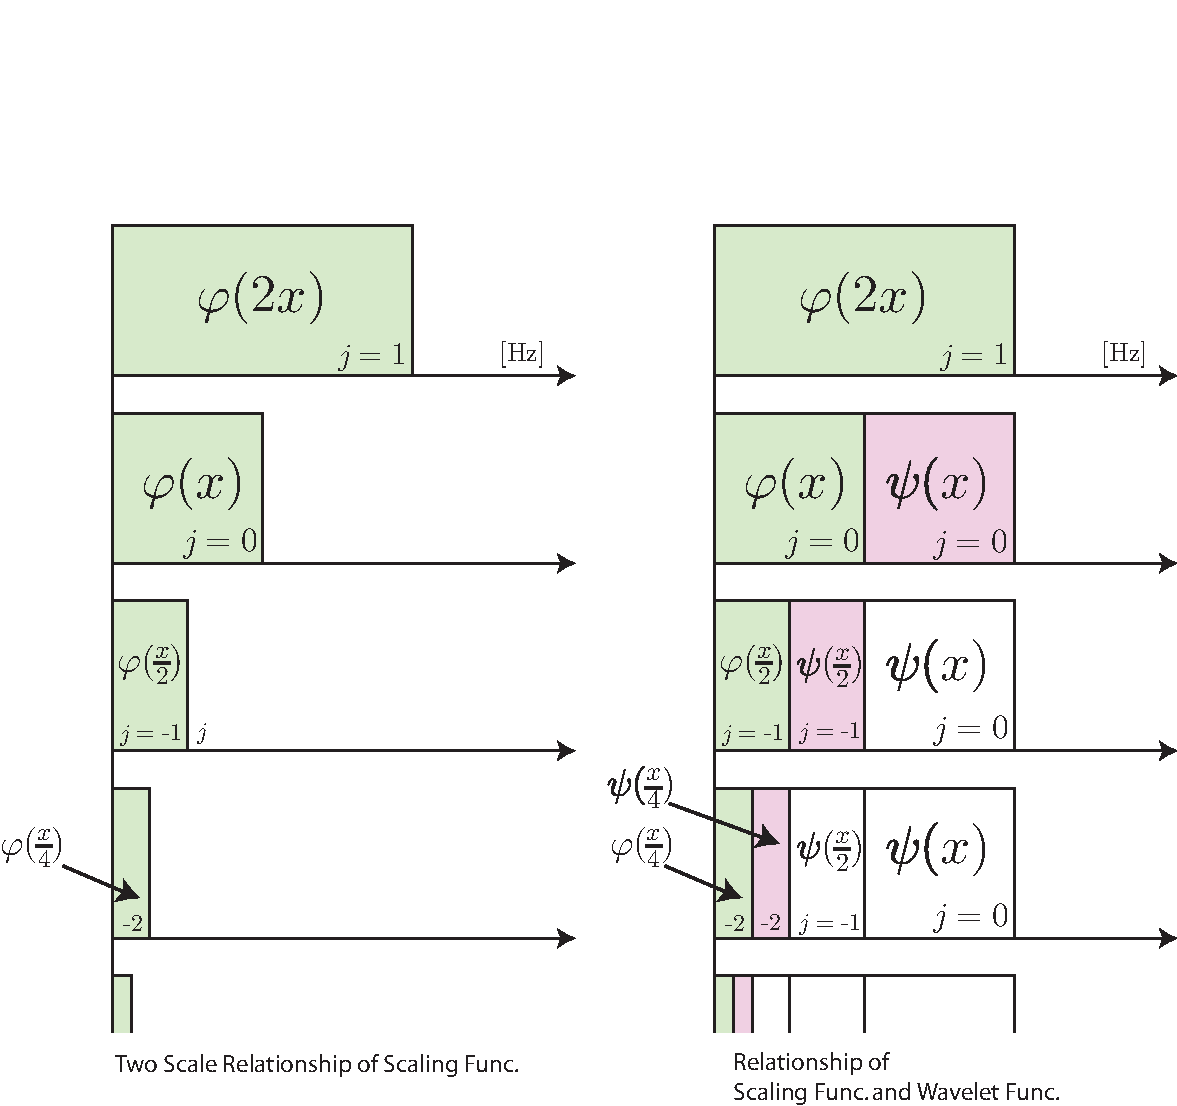
\includegraphics[width=3.5in]{chap1/fig/two-scale.pdf}
\caption{ツースケール関係} \label{fig-two-scale.pdf}
\end{center}
\end{figure}
算術符号は,区間を記号の出現確率に比例した小区間に分割して行くことで符号化を行う.
それでは例として,記号列abbbcを符号化してみる.式(\ref{eqAAAA})をみてね、。

\begin{equation}
S=\sum_{n=0}^N n^2 \label{eqAAAA}
\end{equation}
○○○○○○○○○○○○○○○○○○○○○○○○○ ○○○○○○○○○○○○○○○○○○○○○○○○○○○○○○○○○○○○○○○○○○○○○○○○○○○○○○○○ ○○○○○○○○○○○○○○○○○○○○○○○○○○○○○○○○○○○○○○○○○○○○○○○○○○○○○○ ○○○○○○○○○○○○○○○○○ ○○○○○○○○○○○○○○○○○○○○○○○○○○○○○○○○○○○○○○○○○○○○○○○○○○○○○○○○ ○○○○○○○○○○○○○○○○○○○○○○○○○○○○○○○○○○○○○○○○○○○○○○○○○○○○○○ ○○○
\section{だだだだ}
何か書く○○○○○○○○○○○○○○○○○○○○○○○○○ ○○○○○○○○○○○○○○○○○○○○○○○○○○○○○○○○○○○○○○○○○○○○○○○○○○○○○○○○ ○○○○○○○○○○○○○○○○○○○○○○○○○○○○○○○○○○○○○○○○○○○○○○○○○○○○○○ ○○○○○○○○○○○○○○○○○ ○○○○○○○○○○○○○○○○○○○○○○○○○○○○○○○○○○○○○○○○○○○○○○○○○○○○○○○○
\subsection{あああ} ○○○○○○○○○○○○○○○○○○○○○○○○○○○○○○○○○○○○○○○○○○○○○○○○○○○○○○ ○○○
\section{だああああ}
何か書く○○○○○○○○○○○○○○○○○○○○○○○○○ ○○○○○○○○○○○○○○○○○○○○○○○○○○○○○○○○○○○○○○○○○○○○○○○○○○○○○○○○ ○○○○○○○○○○○○○○○○○○○○○○○○○○○○○○○○○○○○○○○○○○○○○○○○○○○○○○ ○○○○○○○○○○○○○○○○○ ○○○○○○○○○○○○○○○○○○○○○○○○○○○○○○○○○○○○○○○○○○○○○○○○○○○○○○○○ ○○○○○○○○○○○○○○○○○○○○○○○○○○○○○○○○○○○○○○○○○○○○○○○○○○○○○○ ○○○


\subsection{基本的な考え方}
まず「算術符号」の{\gt 基本的な考え方について説明}する\cite{wavelet-2}.
算術符号は記号列,もしくは{\huge 文字列全体を\gt ひとつの符号語に}する方法であり,1960年代にP.Eliasによって提案された.\par
算術符号は,記号列を実数0と1の間の区間を用いて表す.たとえば,記号は{a,b,c}の3種類があり,
出現確率をそれぞれP(a) = 0.2,P(b) = 0.6,P(c) = 0.2とする.
算術符号は,区間を記号の出現確率に比例した小区間に分割して行くことで符号化を行う.
ここからは節\ref{QWERT}を参照してください。
それでは例として,記号列abbbcを符号化してみる.


\section{算術符号化}
sdssddsfsdds





\begin{figure}[htbp]
\begin{center}
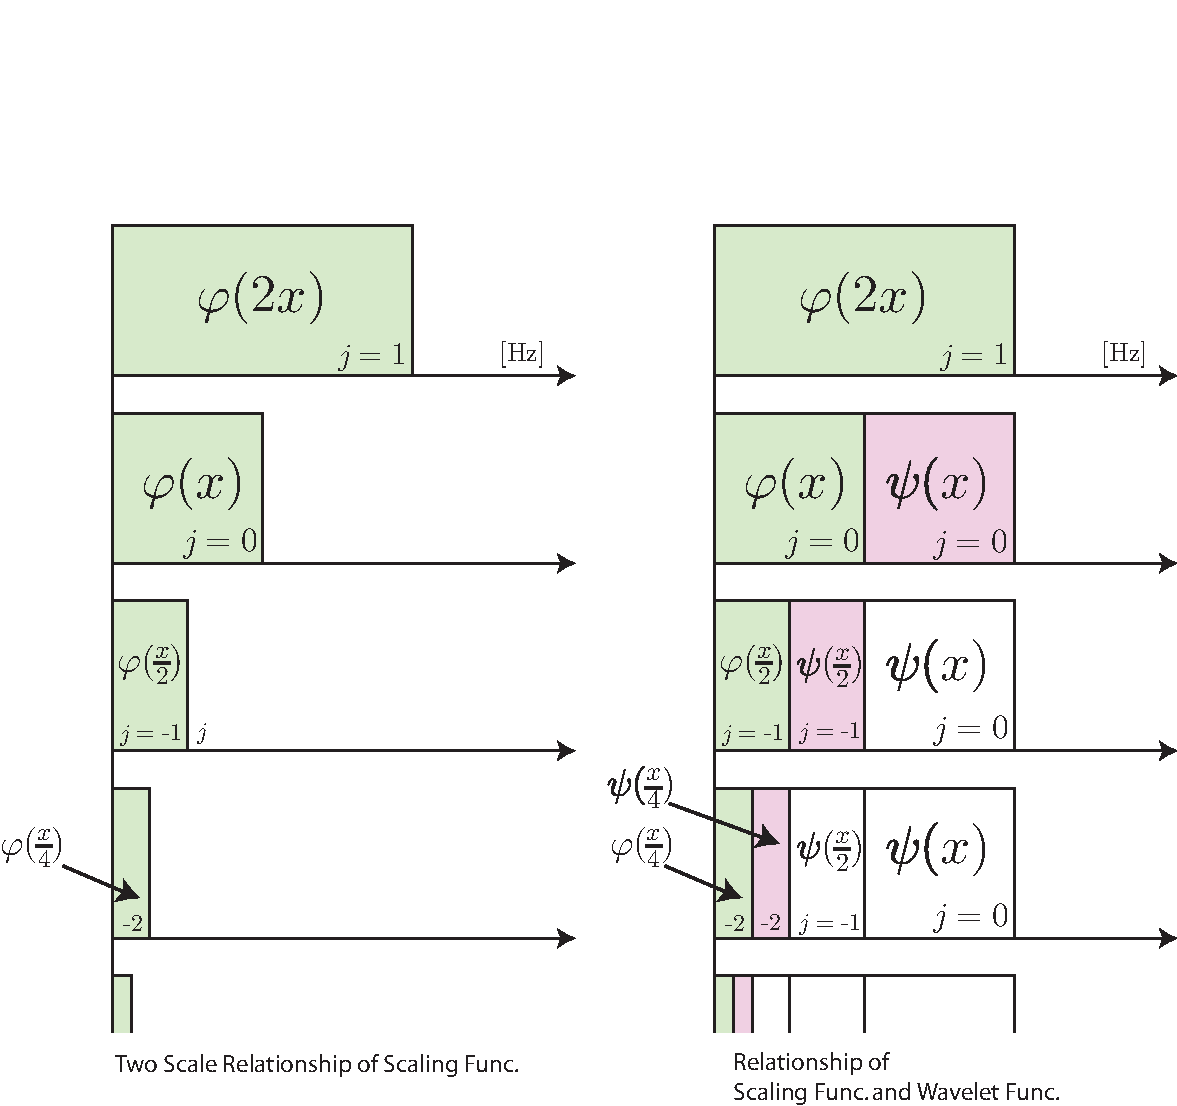
\includegraphics[width=3in]{chap1/fig/two-scale.pdf}
\caption{ツースケール関係aassad} \label{fig-two-scale.pdf}
\end{center}
\end{figure}

図\ref{fig-two-scale.pdf}に●●●を示す.


%% 大きなテーブルをいれるサンプル(longtable)
\begin{table}[h]
\begin{center}
\caption{言語別の特色}\label{AAB}
\begin{longtable}{|l|l|}
\hline
言語 & 特色 \\
\hline
MySQL & あああああああああああああああああああああああ \\
\hline
Oracle & いいいいいいいいいいいいいいいいいい \\
\hline
SQL Server & ううううううううううううううううううう \\
 \hline
\end{longtable}
\end{center}
\end{table}



\subsection{平均符号長} \label{fugocho}
表\ref{tab:scores}に○○○を示す。リスト\ref{test.rb}に○○○を示す。


%%%%%%%%%%%% 図の挿入 %%%%%%%%%%%%%
\begin{figure}[htbp]
\centering
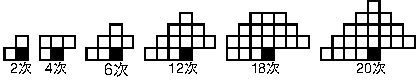
\includegraphics[width=\textwidth]{chap2/fig/tiger.pdf}
\caption{トラがでた}
\end{figure}

%%%%%%%%%%%% 数式
ベクトル$\bm{x}$とただの$x_0$
\begin{equation}
1+1 \C{うわあー!}
\end{equation}

%%%%%%%%%%%% 大きさをかえる
\scalebox{25.0}
{
あ
}
%
\begin{table}[htbp]
\caption{aaa}
\scalebox{5.0}
{
\begin{tabular}{cc}
あ & い \\ \hline
え  & お \\ \hline
\end{tabular}
}
\end{table}
 % 2章
% !TeX root = paper.tex


\chapter{システム構成}\label{genri}
あわれといふも,なかなか疎かなり.されば,人間の儚き事は,老少不定のさかいなれば,誰の人も早く後生の一大事を心にかけて,阿弥陀仏を深く頼み参らせて,念仏申すべきものなり. あなかしこ,あなかしこ.

\section{だああああ}
bababbaba
 % 3章
% !TeX root = paper.tex


\chapter{実験}
あわれといふも,なかなか疎かなり.されば,人間の儚き事は,老少不定のさかいなれば,誰の人も早く後生の一大事を心にかけて,阿弥陀仏を深く頼み参らせて,念仏申すべきものなり. あなかしこ,あなかしこ.ああわれといふも,なかなか疎かなり.されば,人間の儚き事は,老少不定のさかいなれば,誰の人も早く後生の一大事を心にかけて,阿弥陀仏を深く頼み参らせて,念仏申すべきものなり. あなかしこ,あなかしこ.われといふも,なかなか疎かなり.されば,人間の儚き事は,老少不定のさかいなれば,誰の人も早く後生の一大事を心にかけて,阿弥陀仏を深く頼み参らせて,念仏申すべきものなり. あなかしこ,あなかしこ.
 % 4章
% !TeX root = paper.tex


\chapter{結論}
あわれといふも,なかなか疎かなり.されば,人間の儚き事は,老少不定のさかいなれば,誰の人も早く後生の一大事を心にかけて,阿弥陀仏を深く頼み参らせて,念仏申すべきものなり. あなかしこ,あなかしこ.あわれといふも,なかなか疎かなり.されば,人間の儚き事は,老少不定のさかいなれば,誰の人も早く後生の一大事を心にかけて,阿弥陀仏を深く頼み参らせて,念仏申すべきものなり. あなかしこ,あなかしこ.あわれといふも,なかなか疎かなり.されば,人間の儚き事は,老少不定のさかいなれば,誰の人も早く後生の一大事を心にかけて,阿弥陀仏を深く頼み参らせて,念仏申すべきものなり. あなかしこ,あなかしこ.あわれといふも,なかなか疎かなり.されば,人間の儚き事は,老少不定のさかいなれば,誰の人も早く後生の一大事を心にかけて,阿弥陀仏を深く頼み参らせて,念仏申すべきものなり. あなかしこ,あなかしこ.あわれといふも,なかなか疎かなり.されば,人間の儚き事は,老少不定のさかいなれば,誰の人も早く後生の一大事を心にかけて,阿弥陀仏を深く頼み参らせて,念仏申すべきものなり. あなかしこ,あなかしこ.あわれといふも,なかなか疎かなり.されば,人間の儚き事は,老少不定のさかいなれば,誰の人も早く後生の一大事を心にかけて,阿弥陀仏を深く頼み参らせて,念仏申すべきものなり. あなかしこ,あなかしこ.
 % 5章

% !TeX root = paper.tex


\renewcommand{\bibname}{参考文献}
%\addcontentsline{toc}{chapter}{\protect\numberline{参考文献}}
%\addcontentsline{toc}{chapter}{参考文献}
\begin{thebibliography}{99}
\bibitem{1}V.D. Vaughen and T.S. Wilkinson, ''System considerations for
	multispectral image compression designs,'' IEEE Signal
	Process. Mag., vol.12, no.1, pp. 19-31, Jan. 1995.
\bibitem{2}A. Said and W. Pearlman, ''An image multiresolution representation
	for lossless and lossy compression,'' IEEE Trans. Image
	Process., vol.5, no.9, pp.1303-1310, Sept. 1996.
\bibitem{3}小野文孝, ''静止画符号化の新国際標準方式(JPEG2000)の概要,''映
	像情報メディア学会誌, vol.54, no.2, pp.164-171, Feb. 2000.
\bibitem{4}D. Tretter and C.A. Bouman, ''Optimum transform for multispectral
	and multilayer image coding,'' IEEE Trans. Image Process., vol.4, no.3, pp.296-308,
	March 1995.
\bibitem{5}F. Amato, C. Galdi and G. Poggi, ''Embeded zerotree wavelet
	coding on multispectral images,'' IEEE Proc. ICIP 97, vol.1, pp.612-615, 1997.
\bibitem{6}B.R. Epstein, R. Hingorani, J.M. Shapiro and
	M. Czigler, ''Multispectral KLT-wavelet data compression for
	Landsat thematic mapper images,'' Proc. Data Compression
	Conf., IEEE Computer Society Press, pp.200-205, 1992.
\bibitem{7}J.M. Shapiro, S.A. Martucci, and M. Czigler, ''Comparison of
	multispectral Landsat imagery using the embeded zerotree
	wavelet(EZW) algorithm,'' DLPO at Image Compress. Appli. \&
	Innovation Workshop, pp.105-113, March 1994. 
\bibitem{8}J.A. Saghri, A.G. Tescher, and J.T. Reagan, ``Practical transform
	coding of multspectral imagery,'' IEEE Signal Process. Mag.,
	vol.12, no.1, pp.32-43, Jan. 1995.
\bibitem{9}J. Lee, ``Optimized quadtree for Karhunen-Loeve transform in
	multispectral image coding,'' IEEE Trans. Image Process., vol.8, no.4,
	pp.453-461, April 1999.
\bibitem{10}B. Brower, B. Gandhi, D. Couwenhouven and C. Smith, ``ADPCM
	for advanced LANDSAT downlink applications,'' in Proc. 27th
	Asilomar Conf. Signals, Systems and Computers, Nov. 1993. 
\bibitem{11}N.D. Memom, K. Sayood and S.S. Magliveras. ,''Lossless compression
	of multispectral image data,'' IEEE Trans. Geosci. and
	Remote Sensing., vol.32, no.2 , pp.282-289, March 1994.
\bibitem{12}S. Gupta and A. Gersho, ``Feature predictive vector quantization
	of multispectral images,'' IEEE Trans. Geosci. and
	Remote Sensing., vol.30, no.3, pp.491-501, May 1992.
\bibitem{13}K. Irie and R. Kishimoto, ``A study on perfect reconstructive
	subband coding,'' IEEE Trans. Circuits Syst. Video Technol.,
	vol.1, no.1 , pp.42-48, March 1991.
\bibitem{14} 小松 邦紀, 瀬崎 薫, 安田 靖彦, ``濃淡画像の可逆的なサブ
	バンド符号化法'', 信学論(D-II), vol.J78-D-II, no.3,
	pp.429-436, March 1995.
\bibitem{15}A.R. Calderbank, I. Daubechies, W. Sweldens and B. Yeo, ''Lossless
	image compression using integer to integer wavelet transforms,'' 
	IEEE Proc. ICIP 97, vol.1, pp.596-599, 1997.

\bibitem{16}F.A.M.L. Bruekers and A.W.M.V.D. Enden, ``New networks for
	perfect inversion and perfect reconstruction,'' IEEE
	J. Sel. Areas Commun., vol.10, no.1, pp.130-137,
	Jan. 1992. 
%ブリューカとエンデン「ラダー回路による可逆変換」

\bibitem{17}小松 邦紀, 瀬崎 薫, ``可逆的離散コサイン変換とその画像情報圧
	縮への応用,'' 信学技報, vol.IE97-83, pp.1-6, Nov. 1997.
\bibitem{18}K. Komatsu and K. Sezaki, ''Design for lossless block
	transforms and filter banks for image coding,'' IEICE
	Trans. Fundamentals, vol.E82-A, no.8, pp.1656-1664,
	Aug. 2000.
\bibitem{19}福間 慎治, 岩橋 雅宏, 神林 紀嘉, ``可逆的色変換を用いた色彩
	画像の可逆符号化,'' 信学論(D-II), vol.J81-D-II, no.11, pp.2680-2684, Nov. 1998.
\bibitem{20} T. Nakachi, T. Fujii, and J. Suzuki,''A unified coding
	algorithm of lossless and near-lossless color image
	compression,'' IEICE Trans. Fundamentals, vol.E83-A, no.2,
	pp. 301-310, Feb. 2000.
\bibitem{21}仲地 孝之, 藤井 竜也, ``可逆KL変換を用いた病理顕微鏡画像符号
	化法の研究,'' 2000信学総大, D16-13, March 2000.
\bibitem{22}鷹合 大輔, 武部 幹, ``可逆WT・KLTを用いるマルチスペクトル画
	像の情報圧縮,'' 信学論(A), vol.J84-A, no.3, pp.1-11, March
	2001.
\bibitem{23}尾上 守夫, ``画像処理ハンドブック,'' 昭晃堂, pp.554-561, 1987.
\bibitem{24}鷹合 大輔, 武部 幹, ``マルチスペクトル画像のバンド間・バンド
	内相関除去による可逆情報圧縮,'' 第15回DSPシンポジウム講演論文集, pp.475-48, Nov.
	2000.
\bibitem{25}鷹合 大輔, 武部 幹, ``ウェーブレット変換を用いたマルチスペク
	トル画像の情報圧縮符号化法の研究,'' 平成10年度金沢工大卒業論文,
	1998.
\bibitem{26}酒井 幸市,``デジタル画像処理入門,'' コロナ社,1997.
\bibitem{27}榊原 進,``ウェーブレットビギナーズガイド,'' 電機大出版局,
	 1995.
\bibitem{28}武部 幹,``情報圧縮、通信と回路理論,'' 信学技報,IT97-40,July
	1997.
\bibitem{29}Gilbert Strang and Troung Nguyen,``
Wavelet and filter banks,' 'Wellesly Cambridge Press,1996.
\bibitem{30}貴家 仁志,``よくわかるディジタル画像処理,'' CQ出版社,1996.
\bibitem{bk1} "金沢の暮らし", \url{http://www.kanazawa-it.ac.jp}
\bibitem{bk2} 山田 太郎, "金沢の一人暮らし", トンチンカン出版, 2016.
 \end{thebibliography}
 
 % 参考文献
\newpage
% !TeX root = paper.tex


\appendix %付録
\chapter{開発したプログラム}
\section{セットアップ方法}


にプログラムの使い方,セットアップ方法などを書きましょう.ここにプログラここにプログラムの使い方,セットアップ方法などを書きましょう.ムの使い方,セットアップ方法などを書きましょう.
ここにプログラムの使い方,セットアップ方法などを書きましょう.

\begin{Verbatim}[frame=single]
$ sudo apt-get install python3-pip      # PIPコマンドの導入
$ echo "Hello WOrld"
Hello WOrld
\end{Verbatim}

にプログラムの使い方,セットアップ方法などを書きましょう.ここにプログラここにプログラムの使い方,セットアップ方法などを書きましょう.ムの使い方,セットアップ方法などを書きましょう.
ここにプログラムの使い方,セットアップ方法などを書きましょう.

\section{使い方}
ここにプログラムの使い方,セットアップ方法などを書きましょう.
ここにプログラムの使い方,セットアップ方法などを書きましょう.ここにプログラここにプログラムの使い方,セットアップ方法などを書きましょう.ムの使い方,セットアップ方法などを書きましょう.
ここにプログラムの使い方,セットアップ方法などを書きましょう.ここにプログラムの使い方,セットアップ方法などを書きましょう.
%%%%%%%%%%%%% プログラムの埋め込み %%%%%%%%%%%%%%%%%%%%%%%%%

\section{ソースコード}
%% ファイル名を指定して、挿入する場合
\lstinputlisting[language=c,caption=サンプルプログラム,label=sample.c]{appendix/src/sample.c}

%% 直接プログラムを埋め込む場合
\begin{lstlisting}[language=ruby,caption=スパゲッティソース,label=test.rb]
#! /usr/local/bin/ruby -Ks
# numbers.rb
print "正の整数値を表す文字列を入力してください。正の整数値を表す文字列を入力してください。\n"
while true
	print ">"
	line = gets.chomp # 改行コードを切り捨てる
	break if line.empty?
	begin
		v = Integer(line) # 文字列を整数化する
	rescue
		puts "変換できません。"
		next
	end
	printf ("2進法:%b\n",v)
	printf ("8進法:%o\n",v)
	printf ("10進法:%d\n",v)
	printf ("16進法:%x\n",v)
end
puts "Bye."
\end{lstlisting}
\chapter{いいいいい}
あああああああああああああああああああああいいいいいいいいいいいいいいいいいいいいいいいいいいいいううううううううううううううううう
     % 付録

\end{document}
